% !TeX root = ../../manuscript.tex
\section{Results and discussion}

\subsection{Equilibration of the trajectories}
In this section, the equilibration of the protein during the various (cosolvent) \gls{md} trajectories is examined by plotting the \gls{rmsd} distance of the protein structure from its initial state throughout the simulated time.
On top of the usual task of selecting the equilibrated part of each trajectory to be considered for further analysis, these plots are useful to detect potential differences in the equilibration process between the traditional and the cosolvent trajectories.
On Figure \ref{fig:rmsd_equilib}, such plots obtained for the first replica of each solvent type are shown.
It is reassuring, that the protein structures seem to be well equilibrated after 50 ns of simulation time in all three cases.
The equilibration appears to be happening slightly faster in the benzene and especially in the phenol cosolvent trajectory than in water.
The equilibrated \gls{rmsd} values plotted on Figure \ref{fig:rmsd_equilib} ar
e somewhat higher for the two cosolvent trajectories than in water.
This could indicate that the cosolvent probes have stabilised some conformatio
ns that are not often visited with water as solvent and that are farther from
the original protein conformation than those appearing frequently in water bas
ed simulations.
\begin{figure}
\centering
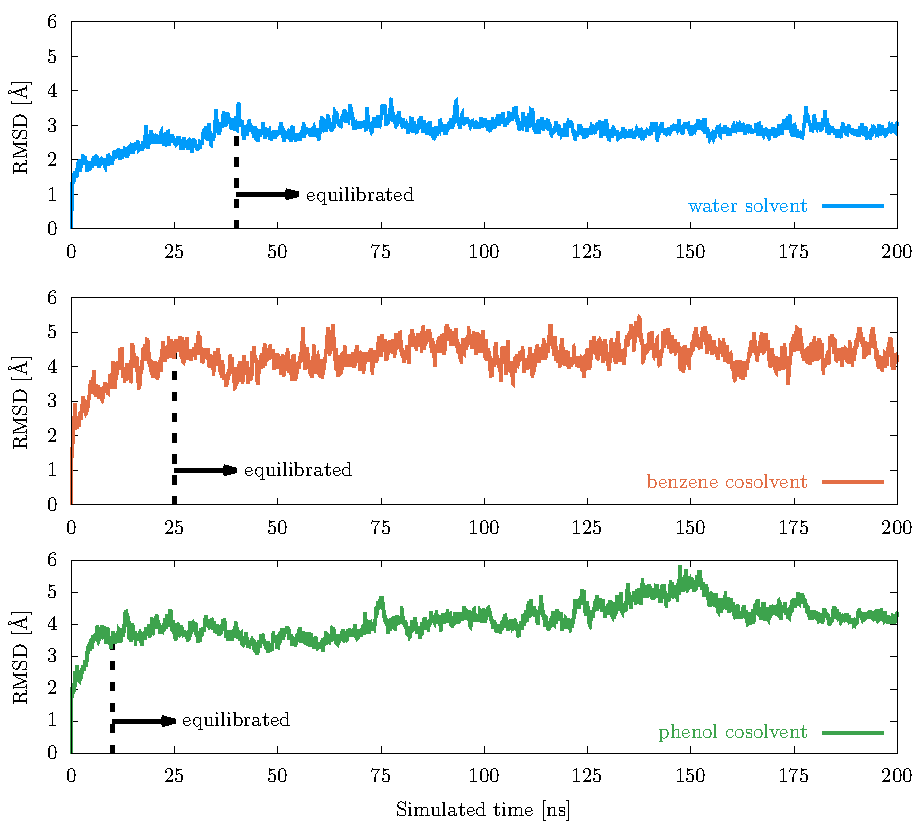
\includegraphics[width=\textwidth]{sections/results/images/rmsd_equilib/to_pdf/rmsd_equilib_to_pdf.pdf}
\caption{The evolution of the \gls{rmsd} distance of the protein from the starting conformation during the \gls{md} trajectories. The first replica for each solvent is plotted.}
\label{fig:rmsd_equilib}
\end{figure}

\subsection{Selecting representative protein conformations}
As mentioned in the Computational Details, the \texttt{dbscan} algorithm of \texttt{cpptraj} is used to perform the clustering of the trajectories.
The clustering is carried out separately for the three solvents, with the three replicas of each of them concatenated and treated as a single trajectory.
In order to carry out a successful clustering of the trajectories, first the $k$ and $\varepsilon$ parameters of the density based clustering algorithm have to be tuned.
On top of performing this tuning of the parameters, the effects of considering only the alpha carbon atoms for the \gls{rmsd} calculations instead of all heavy atoms of the protein are also evaluated.
Finally, possible redundancies in the set of representative protein structures are investigated.

The tuning of the parameters of the \texttt{dbscan} algorithm is performed by systematically varying the values for these parameters to see which combination yields the most optimal clustering.
% Additionally, clustering based only on the \gls{rmsd}s of alpha carbon atoms is compared with all heavy atom \gls{rmsd} clustering.
% The parameter $k$ is varied between four and seven, as the authors of \texttt{cpptraj} write in the User's Manual \cite{amberhub}, that values lower than four do not usually result in any improvements, while the value of of seven is already clearly inferior.
% The other parameter $\varepsilon$ is varied from 0.95 \AA{} to 1.3 \AA{} in the case of alpha carbon clustering, and from 1.3 \AA{} to 1.6 \AA{} when all heavy atoms are considered.
The computation of the \gls{rmsd} distance between all frames of a trajectory is much more demanding if on top of the alpha carbons, all other heavy atoms are considered as well.
To speed up these computations, the technique of sieving is utilised: only every other frame is considered explicitly during the clustering, the remaining frames are simply added to the cluster with the cluster representative most similar to them.
To measure the quality of the clustering four metrics are utilised.
Two of these have already been discussed, namely the \gls{dbi} and the \gls{psf}.
Since both of these scores are heavily influenced by the number of obtained clusters \cite{cluster_perf}, the comparison of their absolute values between different \gls{md} trajectories has limited meaning.
Instead, the trends arising in these metrics through the systematic variation of the clustering parameters can be interpreted to optimise these parameters.
At this point it is useful to reiterate, that low values of \gls{dbi} and high values of \gls{psf} are desirable.
The other two descriptors utilised to describe the quality of the clustering are the number of noise frames (frames not included in any cluster), and the number of clusters defined by the algorithm.
The number of noise frames should clearly be kept low to avoid missing any important conformations, only because it is visited very rarely and is therefore considered an outlier by the algorithm.
Finally, while a high number of clusters is desirable as it can result in a wider variety of protein conformations, the computational limitations of performing explicit docking calculations to each representative conformation with thousands of ligands should be kept in mind.

On Figure \ref{fig:water_clustering_ca}, the descriptors of the water trajectory clustering can be seen, for the case when only the alpha carbons are considered during the \gls{rmsd} distance calculations.
Considering the top two plots at first, it can be observed that the \gls{dbi} and \gls{psf} values are zero if $\varepsilon$ is greater than or equal to 1.2 \AA{}.
The reason for this is that above this $\varepsilon$ value all frames of the trajectory are grouped into a single cluster, for which these descriptors cannot provide a meaningful value.
Since a single cluster is clearly not ideal, these large $\varepsilon$ values do not need to be considered during the search for the optimal parameters.
Focusing instead on parameter $k$, the most significant differences between the different values for this can be discovered on the \gls{psf} plot.
Here, the curves with $k$= 4 or 6, reaching their peak at $\varepsilon$=1.1, are clearly superior to the other two.
The curve corresponding to $k=7$ is somewhat of an outlier on this graph, with its peak \gls{psf} at $\varepsilon$=1.15 \AA{} instead of 1.1 \AA{}.
On the \gls{dbi} plot, the variation of $k$ has much more limited effects.
In fact, all curves are more or less constant if $\varepsilon$ is smaller than or equal to 1.1 \AA{}, at which point the \gls{dbi} values drop rapidly and become zero at 1.2 \AA{}.
Considering that $\varepsilon$=1.1 \AA{} is the point at which the \gls{dbi} values start decreasing, it is reasonable to assume that it is at this point that some significant changes are occurring in the way the clusters are defined.
Together with the fact that $\varepsilon$=1.1 \AA{} provides clusterings with the best \gls{psf} values, this observation makes this value of $\varepsilon$ a promising candidate to be the optimal choice.
By looking at the bottom two plots of Figure \ref{fig:water_clustering_ca}, the number of noise frames and number of clusters can be observed.
On these plots one can find further advantages of the $\varepsilon$=1.1 \AA{} choice.
These are that the number of noise frames start their rapid increase only at slightly smaller epsilon values, and that a reasonable number of clusters, thirteen, are obtained for this value.
\begin{figure}
\centering
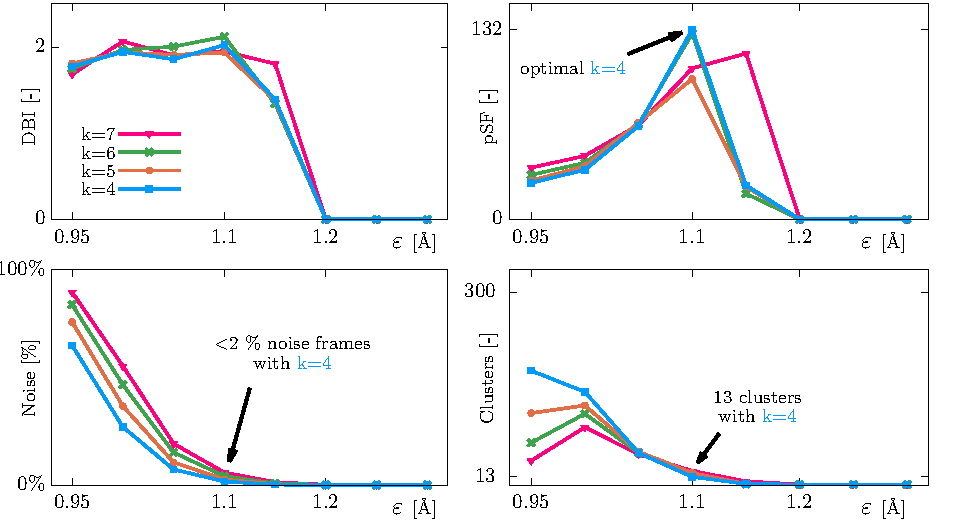
\includegraphics[width=\textwidth]{sections/results/images/water_clustering_ca/to_pdf/water_clustering_ca_to_pdf.pdf}
\caption{Plots of the clustering descriptors utilised for the tuning of the  \texttt{dbscan} parameters.
The descriptors were obtained by clustering the \gls{md} trajectory with water as the solvent and considering only the alpha carbon atoms for the \gls{rmsd} calculations.
The $\varepsilon$ parameter in units of \aa{}ngstr\"oms are shown on the horizontal axes in all cases, while on the vertical axes the various unitless descriptors are shown.
From the top left in clockwise direction: the Davies--Bouldin index, the pseudo-F statistic, the number of clusters and the number of noise frames are shown.}
\label{fig:water_clustering_ca}
\end{figure}

